\documentclass[8pt]{extarticle}
\title{Econ 250 HW 4}
\author{Avinash Iyer}
\date{September 28, 2022}

%font setup
%
%\usepackage[math]{anttor}

%paper setup
\usepackage{geometry}
\geometry{letterpaper, portrait, margin=1in}
\usepackage{fancyhdr}

%symbols
\usepackage{amsmath}
\usepackage{amssymb}
\usepackage{hyperref}
\usepackage{gensymb}

\usepackage[T1]{fontenc}
\usepackage[utf8]{inputenc}

%chemistry stuff
\usepackage[version=4]{mhchem}
\usepackage{chemfig}

%plotting
\usepackage{pgfplots}
\usepackage{tikz}

%\usepackage{natbib}

%graphics stuff
\usepackage{graphicx}
\graphicspath{ {./images/} }

%a useful command
\newcommand{\plain}[1]{\textrm{#1}}

%code stuff
%when using minted, make sure to add the -shell-escape flag
%you can use lstlisting if you don't want to use minted
%\usepackage{minted}
%\usemintedstyle{pastie}
%\newminted[javacode]{java}{frame=lines,framesep=2mm,linenos=true,fontsize=\footnotesize,tabsize=3,autogobble,}
%\newminted[cppcode]{cpp}{frame=lines,framesep=2mm,linenos=true,fontsize=\footnotesize,tabsize=3,autogobble,}

\usepackage{listings}
\usepackage{color}
\definecolor{dkgreen}{rgb}{0,0.6,0}
\definecolor{gray}{rgb}{0.5,0.5,0.5}
\definecolor{mauve}{rgb}{0.58,0,0.82}

\lstset{frame=tb,
	language=Java,
	aboveskip=3mm,
	belowskip=3mm,
	showstringspaces=false,
	columns=flexible,
	basicstyle={\small\ttfamily},
	numbers=none,
	numberstyle=\tiny\color{gray},
	keywordstyle=\color{blue},
	commentstyle=\color{dkgreen},
	stringstyle=\color{mauve},
	breaklines=true,
	breakatwhitespace=true,
	tabsize=3
}
\pagestyle{fancy}
\fancyhf{}
\rhead{Avinash Iyer}
\lhead{Econ 250 HW 4}
\begin{document}{
\maketitle 
\section*{Utility Maximization, Computation}
\subsection*{Part A}
\begin{align*}
	100 &= 2X + Y \\
	MRS_{XY} &= \frac{\frac{\partial U}{\partial X}}{\frac{\partial U}{\partial Y}} \\
	&= \frac{\frac{Y^{0.5}}{X^{0.5}}}{\frac{X^{0.5}}{Y^{0.5}}} \\
	&= \frac{Y}{X} \\
	MRS_{XY} &= \frac{P_{X}}{P_{Y}} \\
	\frac{Y}{X} &= \frac{2}{1} \\
	Y &= 2X \\
	100 &= 4X \\
	X_{A} &= 25 \\
	Y_{A} &= 50 \\
	\\
	300 &= 2X + Y \\
	MRS_{XY} &= \frac{\frac{\partial U}{\partial X}}{\frac{\partial U}{\partial Y}} \\
	&= \frac{0.8 \frac{Y^{0.2}}{X^{0.2}}}{0.2 \frac{X^{0.8}}{Y^{0.8}}} \\
	&= \frac{4Y}{X} \\
	MRS_{XY} &= \frac{P_X}{P_Y} \\
	\frac{4Y}{X} &= \frac{2}{1} \\
	4Y &= 2X \\
	X &= 2Y \\
	300 &= 2(2Y) + Y \\
	300 &= 5Y \\
	Y_B &= 60 \\
	X_B &= 120
\end{align*}
\subsection*{Part B}
Consumer C's marginal rate of substitution at her optimal bundle will be equal to $2$ — consumption is optimized when the utility function is tangent to the budget constraint, which occurs when the utility function is tangent to the budget constraint.
\section*{Utility Maximization, Computation, Extension}
\begin{align*}
	MRS_{NR} &= \frac{\frac{\partial U}{\partial N}}{\frac{\partial U}{\partial R}} \\
	&= \frac{2N(R+5)}{N^2} \\
	&= \frac{2(R+5)}{N} \\
	MRS_{NR} &= \frac{P_N}{P_R} \\
	\frac{2(R+5)}{10} &= \frac{P_N}{2} \\
	2R + 10 &= 5P_{N} \\
	50 &= P_N N + P_R R \\
	&= (P_N)(10) + 2R \\
	50 &= 2(2R+10) + 2R \\
	30 &= 6R \\
	R &= 5 \\
	P_N &= \frac{2(R+5)}{5} \\
	&= \frac{2(10)}{5} \\
	P_N &= \boxed{4}
\end{align*}
\section*{Utility Maximization, Computations, Corner Solutions}
\begin{align*}
	MRS_{BD} &= \frac{\frac{\partial U}{\partial B}}{\frac{\partial U}{\partial D}} \\
	&= \frac{1}{B}\\
	MRS_{BD} &= \frac{P_B}{P_D} \\
	\frac{1}{B} &= \frac{2}{P_D} \\
	B &= \frac{P_D}{2}
\end{align*}
Since for any positive value of $P_D$, there is a positive value of $B$ such that $MRS_{BD} = \frac{P_B}{P_D}$, there is always an interior solution.
\begin{center}
	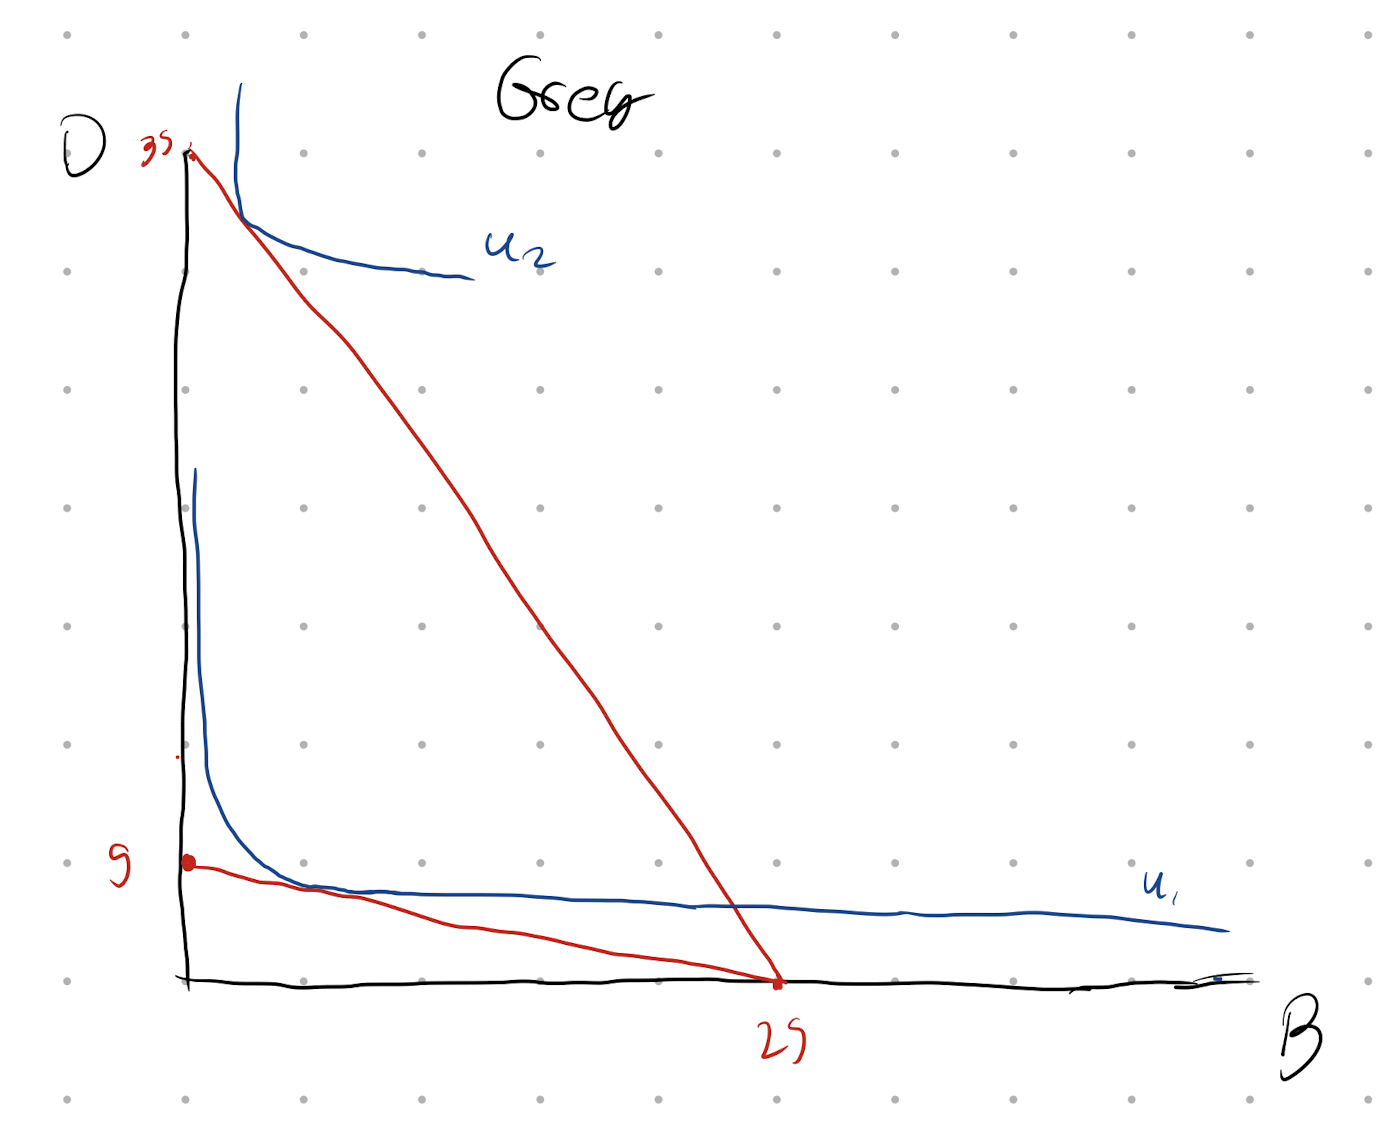
\includegraphics[width=10cm]{HW4Q3}
\end{center}
\section*{Demand Curves}
\begin{align*}
	I &= P_T T + 2S \\
	MRS_{TS} &= \frac{\frac{\partial U}{\partial T}}{\frac{\partial U}{\partial S}} \\
	&= \frac{\frac{1}{T}}{\frac{4}{S}} \\
	&= \frac{S}{4T} \\
	MRS_{TS} &= \frac{P_T}{2} \\
	\frac{S}{4T} &= \frac{P_T}{2} \\
	S &= 2P_T (T) \\
	I &= P_T(T) + 2P_T(T) \\
	T &= \boxed{\frac{I}{3P_T}}
\end{align*}
\section*{Demand and Engel Curves}
\subsection*{Part A}
\begin{center}
	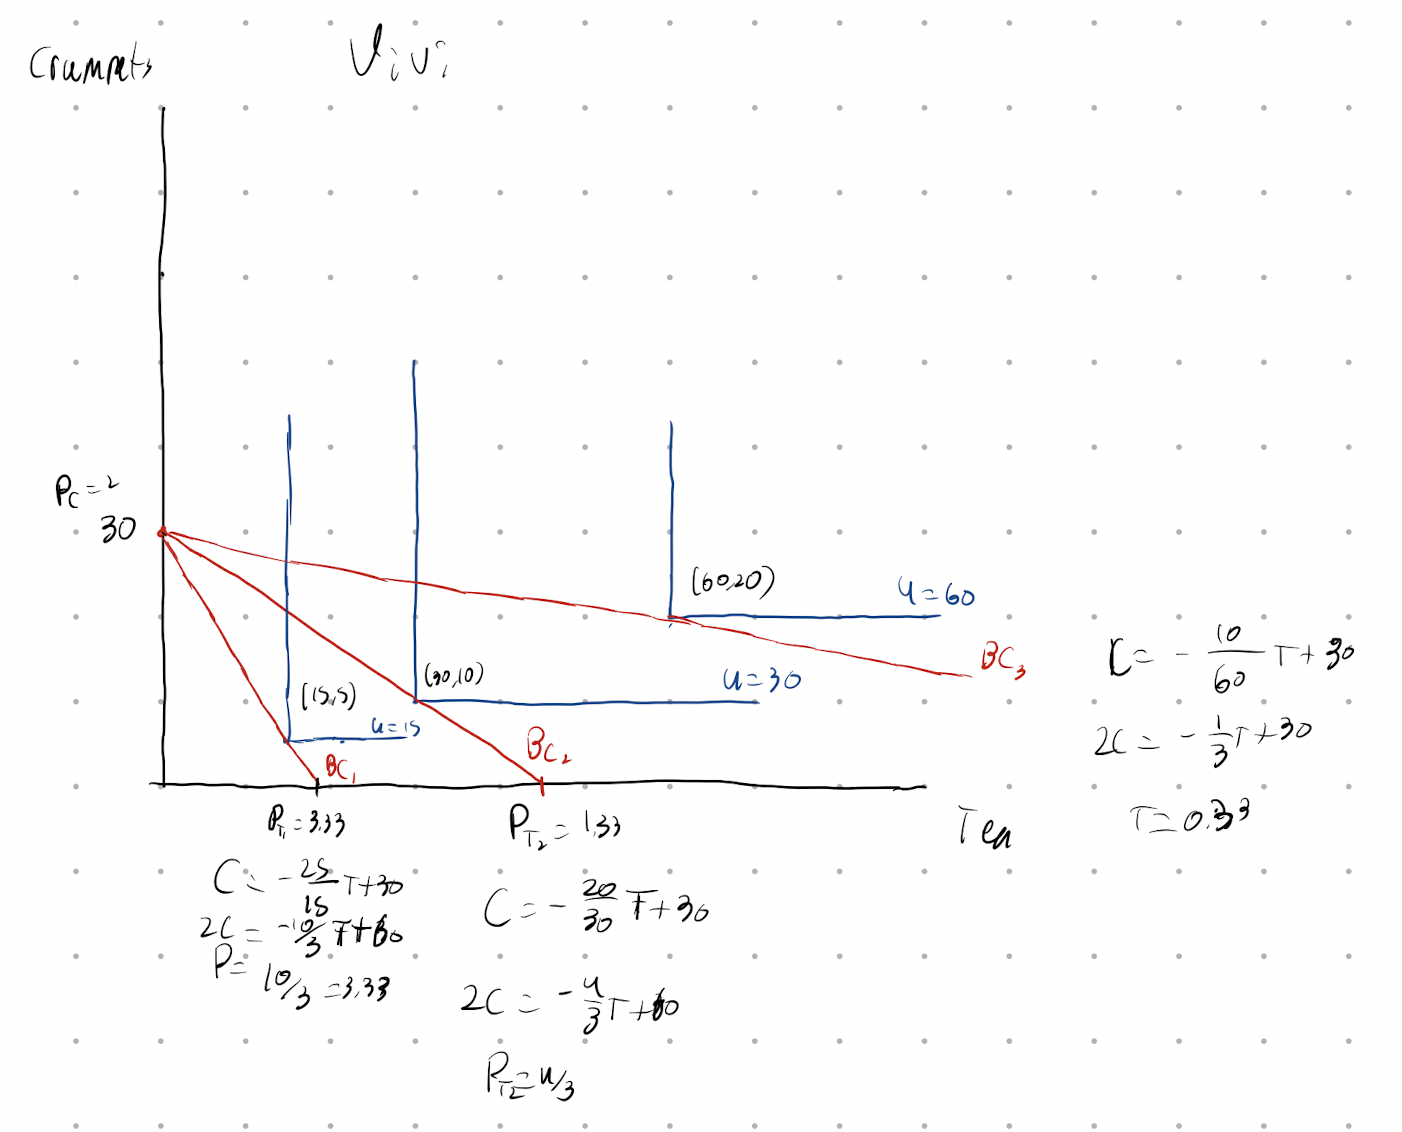
\includegraphics[width=10cm]{HW4Q5AI}
	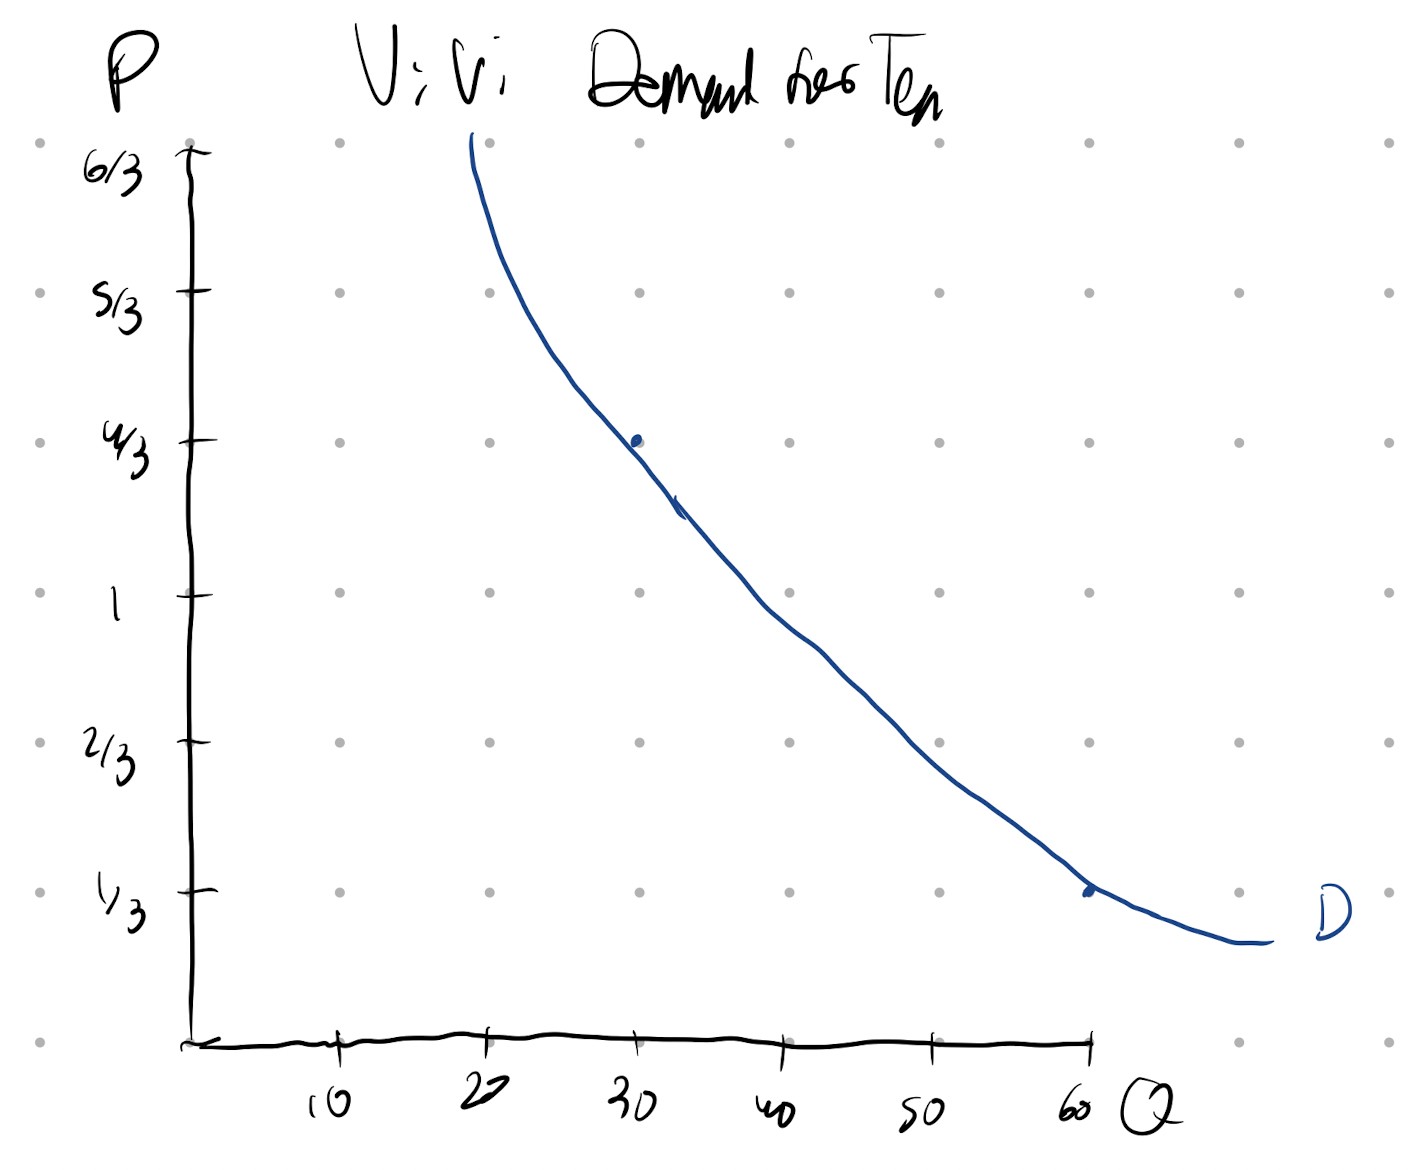
\includegraphics[width=10cm]{HW4Q5AII}
\end{center}
\subsection*{Part B}
\begin{align*}
	60 &= P_T T + P_C C \\
	T &= 3C \\
	60 &= P_T (3C) + P_C C \\
	60 &= (3P_T + P_C) (C) \\
	C &= \boxed{\frac{60}{3P_T + P_C}}
\end{align*}
\section*{Demand and Engel Curves, Quasi-linear Utility}
\subsection*{Part A}
\begin{align*}
	I &= P_C C + P_V V \\
	MRS_{CV} &= \frac{\frac{1}{C}}{2} \\
	&= \frac{1}{2C}\\
	\frac{1}{2C} &= \frac{P_C}{P_V} \\
	P_V &= 2P_C C \\
	C &= \boxed{\frac{P_V}{2P_C}}
\end{align*}
\subsection*{Part B}
\begin{align*}
	I &= P_C C + P_V V \\
	MRS_{CV} &= \frac{\frac{1}{C}}{2} \\
	\frac{1}{2C} &= \frac{P_C}{P_V} \\
	C &= \frac{P_V}{2P_C} \\
	I &= P_C \left(\frac{P_V}{2P_C}\right) + P_V V \\
	I &= \frac{P_V}{2} + P_V V \\
	V &= \boxed{\frac{I}{P_V} - \frac{1}{2}}
\end{align*}
\subsection*{Part C}
\begin{align*}
	C &= \frac{P_V}{2P_C} \\
	&= \frac{8}{8} \\
	&= 1\\
	C &= \begin{cases}
		1, & I \geq 4 \\
		I/4,& 0\geq I < 4
	\end{cases}
\end{align*}
\subsection*{Part D}
For incomes between $0$ and $4$, chocolate ice cream is a normal good, but if income is greater than or equal to $4$, chocolate ice cream is neither normal nor inferior.
\section*{Demand Curves, Linear Utility}
\subsection*{Part A}
\begin{center}
	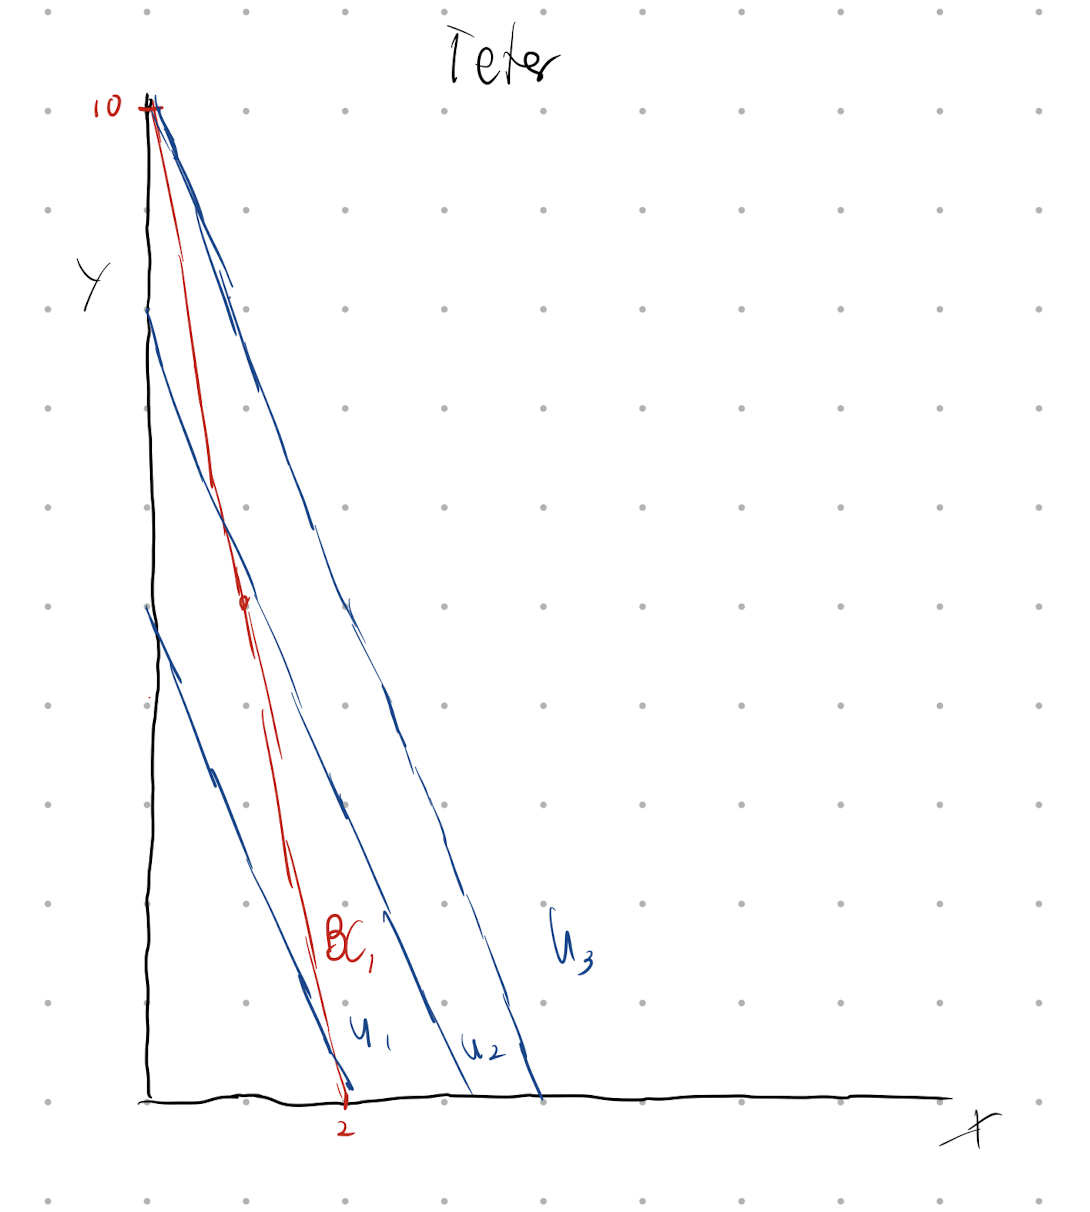
\includegraphics[width=10cm]{HW4Q7A}
\end{center}
Because the market is only willing to offer 1 of good $X$ for every 5 of good $Y$, while he wants 2 of good $X$ for every 5 of good $Y$, he values good $Y$ at a higher level than the market, so his utility is maximized at consuming all of good $Y$.
\subsection*{Part B}
\begin{center}
	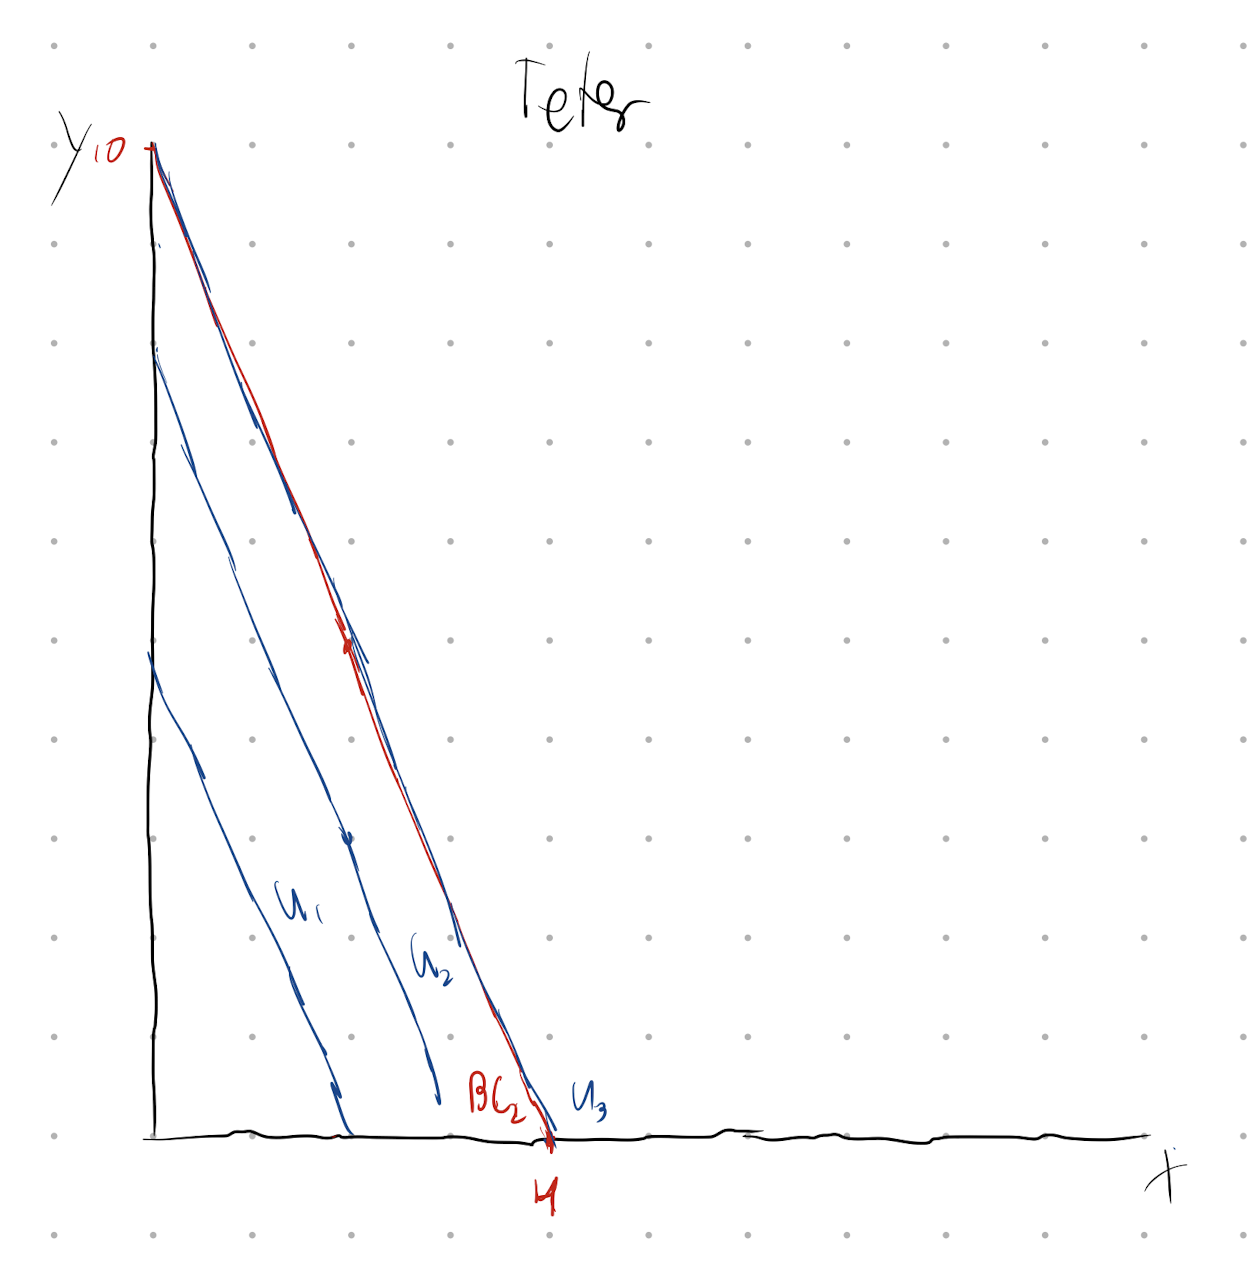
\includegraphics[width=10cm]{HW4Q7B}
\end{center}
Because the market values $Y$ relative to $X$ at the exact same rate as Teter does, every consumption bundle on the budget constraint curve is an optimal consumption bundle.
\subsection*{Part C}
\begin{center}
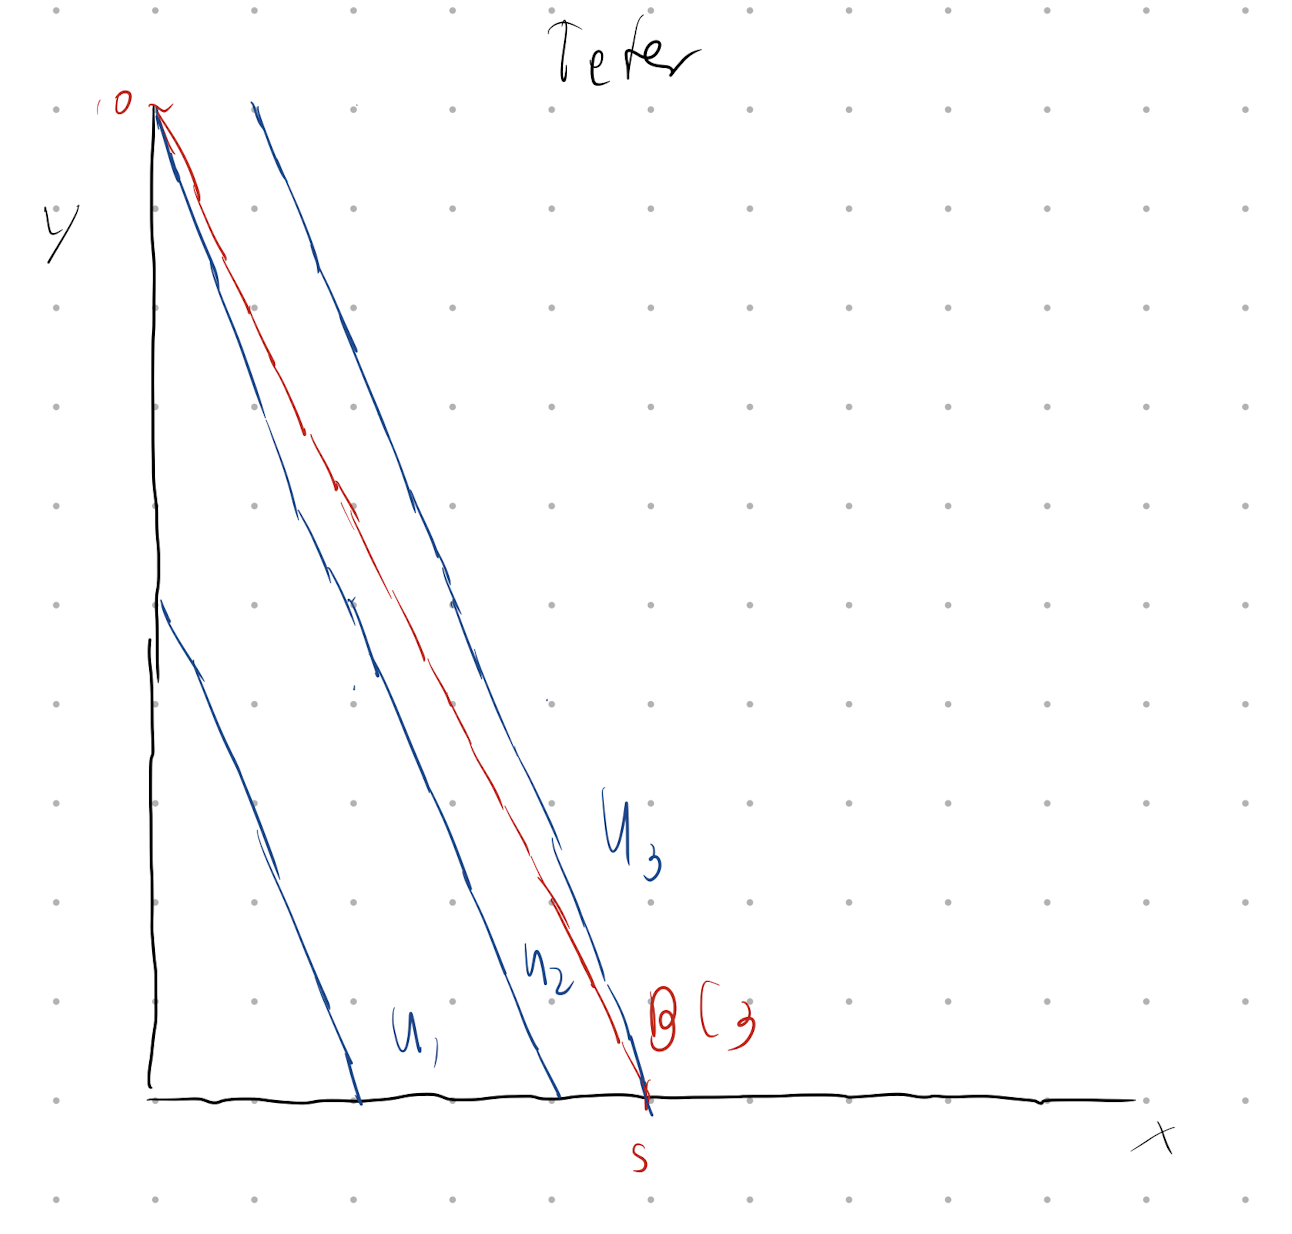
\includegraphics[width=10cm]{HW4Q7C}
\end{center}
Because the market will trade off 2 of good $Y$ in exchange for 1 of good $X$, while Teter will trade off 2.5 of good $Y$ in exchange for 1 of good $X$, his optimal bundle will consist entirely of good $X$.
\subsection*{Part D}
\begin{align*}
	100 &= P_X X + 10Y \\
	MRS_{XY} &= \frac{10}{4} \\
	\frac{10}{4} &= \frac{P_X}{10} \\
	P_X &= 25 \\
	X &= \begin{cases}
		0, & P_X > 25 \\
		[0,4], & P_X = 25 \\
		\frac{100}{P_X}, & 0 < P_X < 25
	\end{cases}
\end{align*}
\subsection*{Part E}
\begin{center}
	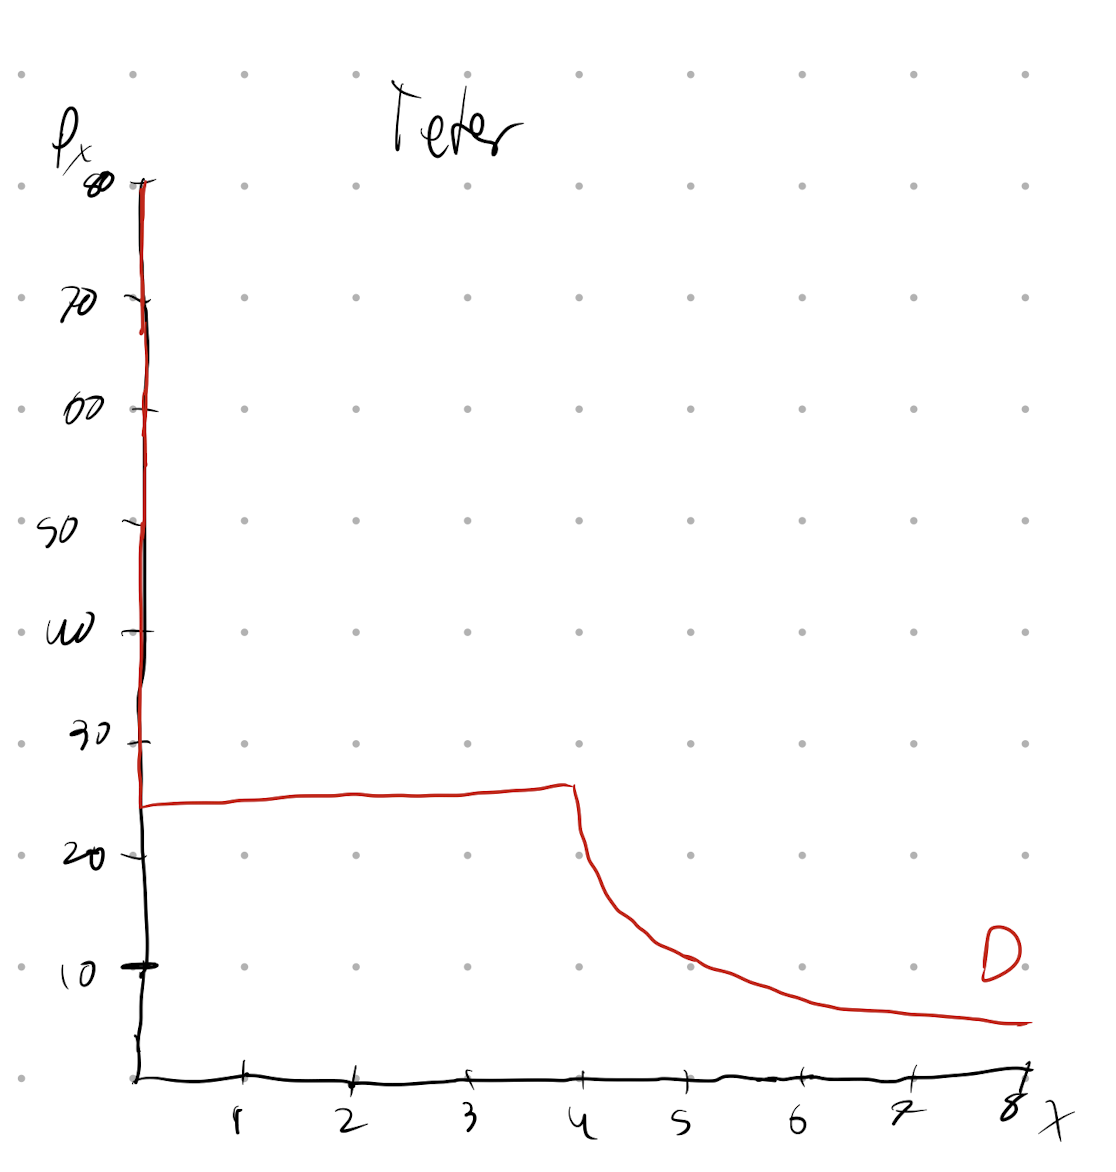
\includegraphics[width=10cm]{HW4Q7E}
\end{center}
\section*{Income and Substitution Effects}
\subsection*{Part A}
\begin{center}
	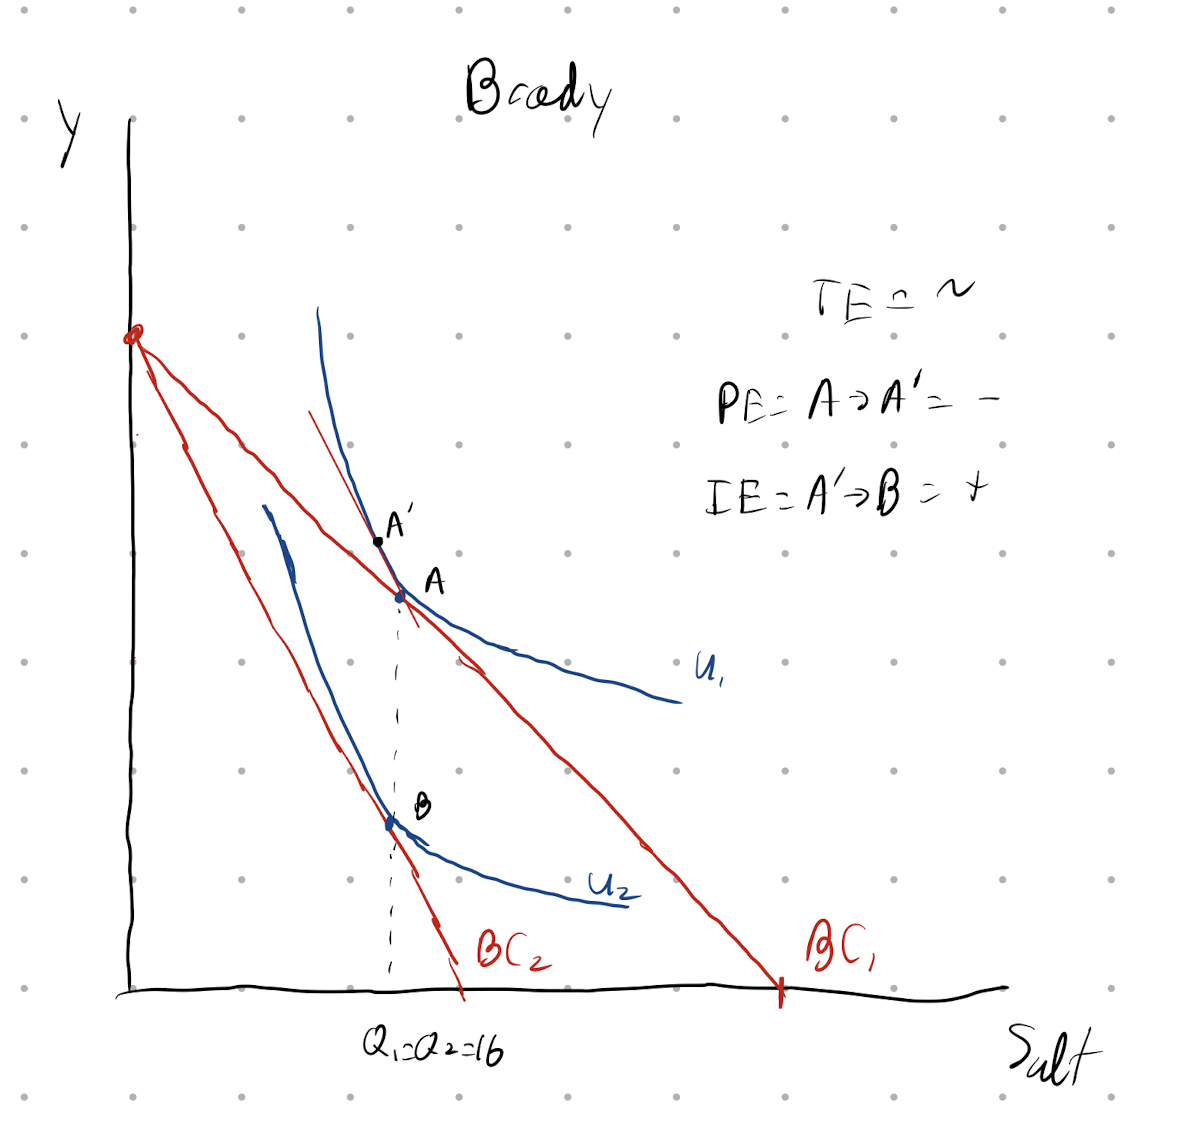
\includegraphics[width=10cm]{HW4Q8A}
\end{center}
Salt is an \textbf{inferior good}, as when the price of salt increased, Brady's relative purchasing power decreased, but his income effect was positive.
\subsection*{Part B}
\begin{align*}
	P_{\plain{own}} &= \frac{\delta\% Q}{\delta \% P} \\
	&= \frac{0}{100} \\
	&= 0
\end{align*}
\subsection*{Part C}
 Since salt is an inferior good, the income elasticity of demand is negative.
\subsection*{Part D}
The substitution and income effects of a change in price of salt are in opposite directions, meaning that if the price of salt goes down, the substitution effect is positive while the income effect is negative, and vice versa.
\section*{Income and Substitution Effects, cont'd}
\begin{center}
	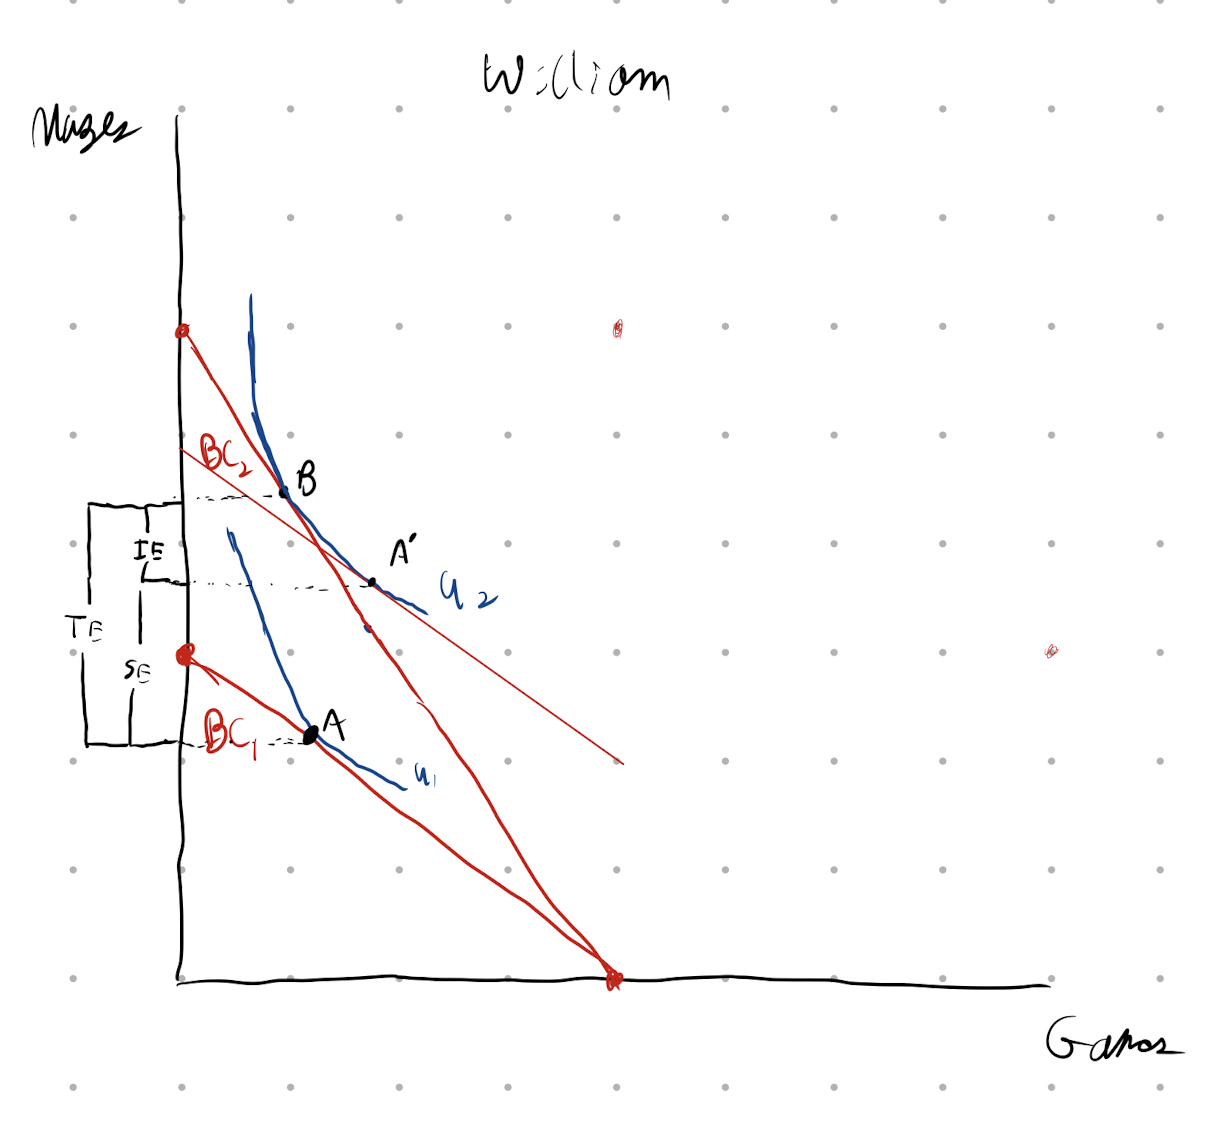
\includegraphics[width=10cm]{HW4Q9}
\end{center}
\section*{Conceptual Questions}
\subsection*{Part A}
True; since the goods are perfect complements, there is no substitution effect, meaning that any increase in the consumption of a good is entirely because of the income effect. Since a decrease in the price of a good leads to increased consumption, these goods are normal goods.
\subsection*{Part B}
False; since the consumption of a good increases as one moves down the demand curve, the utility increases by the principle of non-satiation.
\subsection*{Part C}
True in a narrow sense; since an increase in the price of the diamond would, on one margin, lead to an increase in the consumption of diamonds, diamonds are a Giffen good for Marianne. However, every real life example of a Giffen good is a staple food, so diamonds are not a Giffen good in a real sense for Maurine.
\section*{Combining Supply and Demand}
\begin{align*}
	MRS_{CT} &= \frac{\frac{\partial U}{\partial C}}{\frac{\partial U}{\partial T}} \\
	&= \frac{\frac{1/4 T^{3/4}}{C^{3/4}}}{\frac{3/4 C^{1/4}}{T^{1/4}}} \\
	&= \frac{T}{3C} \\
	\frac{T}{3C} &= \frac{P_C}{P_T} \\
	P_C &= \frac{T}{3C} \\
	T &= 3P_C C\\
	I &= P_C C + P_T T \\
	120 &= P_C C + 3P_C C \\
	120 &= 4P_C C \\
	C &= \frac{30}{P_C} \\
	C_{\plain{dem}} &= kC \\
	40 + 2P_{C} &= k\left(\frac{30}{P_C}\right) \\
	40 + 2(15) &= k\left(\frac{30}{15}\right) \\
	k &= \frac{70}{2} \\
	&= \boxed{35}
\end{align*}

}\end{document}
